\documentclass[twoside]{book}

% Packages required by doxygen
\usepackage{fixltx2e}
\usepackage{calc}
\usepackage{doxygen}
\usepackage[export]{adjustbox} % also loads graphicx
\usepackage{graphicx}
\usepackage[utf8]{inputenc}
\usepackage{makeidx}
\usepackage{multicol}
\usepackage{multirow}
\PassOptionsToPackage{warn}{textcomp}
\usepackage{textcomp}
\usepackage[nointegrals]{wasysym}
\usepackage[table]{xcolor}

% Font selection
\usepackage[T1]{fontenc}
\usepackage[scaled=.90]{helvet}
\usepackage{courier}
\usepackage{amssymb}
\usepackage{sectsty}
\renewcommand{\familydefault}{\sfdefault}
\allsectionsfont{%
  \fontseries{bc}\selectfont%
  \color{darkgray}%
}
\renewcommand{\DoxyLabelFont}{%
  \fontseries{bc}\selectfont%
  \color{darkgray}%
}
\newcommand{\+}{\discretionary{\mbox{\scriptsize$\hookleftarrow$}}{}{}}

% Page & text layout
\usepackage{geometry}
\geometry{%
  a4paper,%
  top=2.5cm,%
  bottom=2.5cm,%
  left=2.5cm,%
  right=2.5cm%
}
\tolerance=750
\hfuzz=15pt
\hbadness=750
\setlength{\emergencystretch}{15pt}
\setlength{\parindent}{0cm}
\setlength{\parskip}{0.2cm}
\makeatletter
\renewcommand{\paragraph}{%
  \@startsection{paragraph}{4}{0ex}{-1.0ex}{1.0ex}{%
    \normalfont\normalsize\bfseries\SS@parafont%
  }%
}
\renewcommand{\subparagraph}{%
  \@startsection{subparagraph}{5}{0ex}{-1.0ex}{1.0ex}{%
    \normalfont\normalsize\bfseries\SS@subparafont%
  }%
}
\makeatother

% Headers & footers
\usepackage{fancyhdr}
\pagestyle{fancyplain}
\fancyhead[LE]{\fancyplain{}{\bfseries\thepage}}
\fancyhead[CE]{\fancyplain{}{}}
\fancyhead[RE]{\fancyplain{}{\bfseries\leftmark}}
\fancyhead[LO]{\fancyplain{}{\bfseries\rightmark}}
\fancyhead[CO]{\fancyplain{}{}}
\fancyhead[RO]{\fancyplain{}{\bfseries\thepage}}
\fancyfoot[LE]{\fancyplain{}{}}
\fancyfoot[CE]{\fancyplain{}{}}
\fancyfoot[RE]{\fancyplain{}{\bfseries\scriptsize Generated on Mon Aug 24 2015 16\+:26\+:37 for Stirling by Doxygen }}
\fancyfoot[LO]{\fancyplain{}{\bfseries\scriptsize Generated on Mon Aug 24 2015 16\+:26\+:37 for Stirling by Doxygen }}
\fancyfoot[CO]{\fancyplain{}{}}
\fancyfoot[RO]{\fancyplain{}{}}
\renewcommand{\footrulewidth}{0.4pt}
\renewcommand{\chaptermark}[1]{%
  \markboth{#1}{}%
}
\renewcommand{\sectionmark}[1]{%
  \markright{\thesection\ #1}%
}

% Indices & bibliography
\usepackage{natbib}
\usepackage[titles]{tocloft}
\setcounter{tocdepth}{3}
\setcounter{secnumdepth}{5}
\makeindex

% Hyperlinks (required, but should be loaded last)
\usepackage{ifpdf}
\ifpdf
  \usepackage[pdftex,pagebackref=true]{hyperref}
\else
  \usepackage[ps2pdf,pagebackref=true]{hyperref}
\fi
\hypersetup{%
  colorlinks=true,%
  linkcolor=blue,%
  citecolor=blue,%
  unicode%
}

% Custom commands
\newcommand{\clearemptydoublepage}{%
  \newpage{\pagestyle{empty}\cleardoublepage}%
}


%===== C O N T E N T S =====

\begin{document}

% Titlepage & ToC
\hypersetup{pageanchor=false,
             bookmarks=true,
             bookmarksnumbered=true,
             pdfencoding=unicode
            }
\pagenumbering{roman}
\begin{titlepage}
\vspace*{7cm}
\begin{center}%
{\Large Stirling \\[1ex]\large 0.\+1 }\\
\vspace*{1cm}
{\large Generated by Doxygen 1.8.10}\\
\vspace*{0.5cm}
{\small Mon Aug 24 2015 16:26:37}\\
\end{center}
\end{titlepage}
\clearemptydoublepage
\tableofcontents
\clearemptydoublepage
\pagenumbering{arabic}
\hypersetup{pageanchor=true}

%--- Begin generated contents ---
\chapter{Hierarchical Index}
\section{Class Hierarchy}
This inheritance list is sorted roughly, but not completely, alphabetically\+:\begin{DoxyCompactList}
\item \contentsline{section}{pempek\+:\+:assert\+:\+:implementation\+:\+:Assert\+Used\+Wrapper$<$ level, T $>$}{\pageref{classpempek_1_1assert_1_1implementation_1_1_assert_used_wrapper}}{}
\item \contentsline{section}{Drawable}{\pageref{class_drawable}}{}
\item exception\begin{DoxyCompactList}
\item \contentsline{section}{pempek\+:\+:assert\+:\+:Assertion\+Exception}{\pageref{classpempek_1_1assert_1_1_assertion_exception}}{}
\end{DoxyCompactList}
\item \contentsline{section}{Program}{\pageref{class_program}}{}
\item \contentsline{section}{pempek\+:\+:assert\+:\+:implementation\+:\+:Static\+Assertion$<$ bool $>$}{\pageref{structpempek_1_1assert_1_1implementation_1_1_static_assertion}}{}
\item \contentsline{section}{pempek\+:\+:assert\+:\+:implementation\+:\+:Static\+Assertion$<$ true $>$}{\pageref{structpempek_1_1assert_1_1implementation_1_1_static_assertion_3_01true_01_4}}{}
\item \contentsline{section}{pempek\+:\+:assert\+:\+:implementation\+:\+:Static\+Assertion\+Test$<$ i $>$}{\pageref{structpempek_1_1assert_1_1implementation_1_1_static_assertion_test}}{}
\item \contentsline{section}{Stirling\+Engine}{\pageref{class_stirling_engine}}{}
\item \contentsline{section}{Window}{\pageref{class_window}}{}
\end{DoxyCompactList}

\chapter{Class Index}
\section{Class List}
Here are the classes, structs, unions and interfaces with brief descriptions\+:\begin{DoxyCompactList}
\item\contentsline{section}{\hyperlink{classpempek_1_1assert_1_1_assertion_exception}{pempek\+::assert\+::\+Assertion\+Exception} }{\pageref{classpempek_1_1assert_1_1_assertion_exception}}{}
\item\contentsline{section}{\hyperlink{classpempek_1_1assert_1_1implementation_1_1_assert_used_wrapper}{pempek\+::assert\+::implementation\+::\+Assert\+Used\+Wrapper$<$ level, T $>$} }{\pageref{classpempek_1_1assert_1_1implementation_1_1_assert_used_wrapper}}{}
\item\contentsline{section}{\hyperlink{class_drawable}{Drawable} }{\pageref{class_drawable}}{}
\item\contentsline{section}{\hyperlink{class_program}{Program} }{\pageref{class_program}}{}
\item\contentsline{section}{\hyperlink{structpempek_1_1assert_1_1implementation_1_1_static_assertion}{pempek\+::assert\+::implementation\+::\+Static\+Assertion$<$ bool $>$} }{\pageref{structpempek_1_1assert_1_1implementation_1_1_static_assertion}}{}
\item\contentsline{section}{\hyperlink{structpempek_1_1assert_1_1implementation_1_1_static_assertion_3_01true_01_4}{pempek\+::assert\+::implementation\+::\+Static\+Assertion$<$ true $>$} }{\pageref{structpempek_1_1assert_1_1implementation_1_1_static_assertion_3_01true_01_4}}{}
\item\contentsline{section}{\hyperlink{structpempek_1_1assert_1_1implementation_1_1_static_assertion_test}{pempek\+::assert\+::implementation\+::\+Static\+Assertion\+Test$<$ i $>$} }{\pageref{structpempek_1_1assert_1_1implementation_1_1_static_assertion_test}}{}
\item\contentsline{section}{\hyperlink{class_stirling_engine}{Stirling\+Engine} }{\pageref{class_stirling_engine}}{}
\item\contentsline{section}{\hyperlink{class_window}{Window} }{\pageref{class_window}}{}
\end{DoxyCompactList}

\chapter{File Index}
\section{File List}
Here is a list of all documented files with brief descriptions\+:\begin{DoxyCompactList}
\item\contentsline{section}{\hyperlink{_drawable_8h}{Drawable.\+h} \\*Generic Draw Class This class is the base level of drawable objects to be sent to open\+G\+L to be rendered }{\pageref{_drawable_8h}}{}
\item\contentsline{section}{\hyperlink{global__includes_8h}{global\+\_\+includes.\+h} \\*Base-\/line header file containing global definitions, includes, and variables }{\pageref{global__includes_8h}}{}
\item\contentsline{section}{{\bfseries G\+L\+S\+L.\+h} }{\pageref{_g_l_s_l_8h}}{}
\item\contentsline{section}{\hyperlink{_main_8cpp}{Main.\+cpp} \\*Main program }{\pageref{_main_8cpp}}{}
\item\contentsline{section}{{\bfseries pempek\+\_\+assert.\+h} }{\pageref{pempek__assert_8h}}{}
\item\contentsline{section}{\hyperlink{_program_8h}{Program.\+h} \\*Header file for includes and definitions on G\+L\+S\+L shader wrapper }{\pageref{_program_8h}}{}
\item\contentsline{section}{\hyperlink{_stirling_engine_8h}{Stirling\+Engine.\+h} \\*Main State header file Includes and definitions to enable a main loop within the engine }{\pageref{_stirling_engine_8h}}{}
\item\contentsline{section}{\hyperlink{_window_8cpp}{Window.\+cpp} \\*\hyperlink{class_window}{Window} wrapper class }{\pageref{_window_8cpp}}{}
\item\contentsline{section}{\hyperlink{_window_8h}{Window.\+h} \\*Wrapper for G\+L\+F\+Wwindow }{\pageref{_window_8h}}{}
\end{DoxyCompactList}

\chapter{Class Documentation}
\hypertarget{classpempek_1_1assert_1_1_assertion_exception}{}\section{pempek\+:\+:assert\+:\+:Assertion\+Exception Class Reference}
\label{classpempek_1_1assert_1_1_assertion_exception}\index{pempek\+::assert\+::\+Assertion\+Exception@{pempek\+::assert\+::\+Assertion\+Exception}}
Inheritance diagram for pempek\+:\+:assert\+:\+:Assertion\+Exception\+:\begin{figure}[H]
\begin{center}
\leavevmode
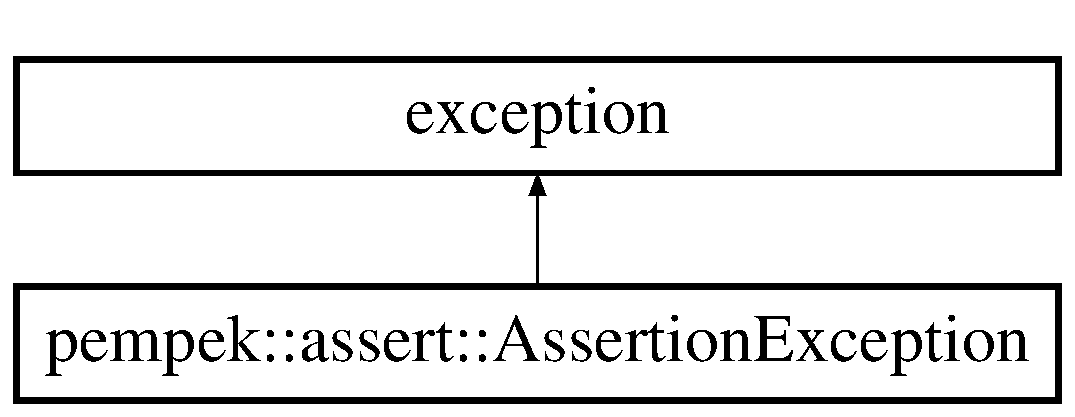
\includegraphics[height=2.000000cm]{classpempek_1_1assert_1_1_assertion_exception}
\end{center}
\end{figure}
\subsection*{Public Member Functions}
\begin{DoxyCompactItemize}
\item 
\hypertarget{classpempek_1_1assert_1_1_assertion_exception_a085718100146da1f43fad9c8ff8a04c3}{}{\bfseries Assertion\+Exception} (const char $\ast$file, int line, const char $\ast$function, const char $\ast$expression, const char $\ast$message)\label{classpempek_1_1assert_1_1_assertion_exception_a085718100146da1f43fad9c8ff8a04c3}

\item 
\hypertarget{classpempek_1_1assert_1_1_assertion_exception_a831b89bd127de1e913f303d9c7fc67e1}{}{\bfseries Assertion\+Exception} (const \hyperlink{classpempek_1_1assert_1_1_assertion_exception}{Assertion\+Exception} \&rhs)\label{classpempek_1_1assert_1_1_assertion_exception_a831b89bd127de1e913f303d9c7fc67e1}

\item 
\hypertarget{classpempek_1_1assert_1_1_assertion_exception_a69433bbae8016750078be991f4076502}{}\hyperlink{classpempek_1_1assert_1_1_assertion_exception}{Assertion\+Exception} \& {\bfseries operator=} (const \hyperlink{classpempek_1_1assert_1_1_assertion_exception}{Assertion\+Exception} \&rhs)\label{classpempek_1_1assert_1_1_assertion_exception_a69433bbae8016750078be991f4076502}

\item 
\hypertarget{classpempek_1_1assert_1_1_assertion_exception_a16600ca18864265781ab4bd24ca0eb8a}{}virtual const char $\ast$ {\bfseries what} () const P\+P\+K\+\_\+\+A\+S\+S\+E\+R\+T\+\_\+\+E\+X\+C\+E\+P\+T\+I\+O\+N\+\_\+\+N\+O\+\_\+\+T\+H\+R\+O\+W\label{classpempek_1_1assert_1_1_assertion_exception_a16600ca18864265781ab4bd24ca0eb8a}

\item 
\hypertarget{classpempek_1_1assert_1_1_assertion_exception_a659fa314977eec7f56fc16601ef30f59}{}const char $\ast$ {\bfseries file} () const \label{classpempek_1_1assert_1_1_assertion_exception_a659fa314977eec7f56fc16601ef30f59}

\item 
\hypertarget{classpempek_1_1assert_1_1_assertion_exception_a4879fdc57b3252b8b04a872215e7c2f3}{}int {\bfseries line} () const \label{classpempek_1_1assert_1_1_assertion_exception_a4879fdc57b3252b8b04a872215e7c2f3}

\item 
\hypertarget{classpempek_1_1assert_1_1_assertion_exception_a020e713ea8d385930d743ff9be017bdf}{}const char $\ast$ {\bfseries function} () const \label{classpempek_1_1assert_1_1_assertion_exception_a020e713ea8d385930d743ff9be017bdf}

\item 
\hypertarget{classpempek_1_1assert_1_1_assertion_exception_aa134ffed2284833917cff6814743fa46}{}const char $\ast$ {\bfseries expression} () const \label{classpempek_1_1assert_1_1_assertion_exception_aa134ffed2284833917cff6814743fa46}

\end{DoxyCompactItemize}


The documentation for this class was generated from the following files\+:\begin{DoxyCompactItemize}
\item 
pempek\+\_\+assert.\+h\item 
pempek\+\_\+assert.\+cpp\end{DoxyCompactItemize}

\hypertarget{classpempek_1_1assert_1_1implementation_1_1_assert_used_wrapper}{}\section{pempek\+:\+:assert\+:\+:implementation\+:\+:Assert\+Used\+Wrapper$<$ level, T $>$ Class Template Reference}
\label{classpempek_1_1assert_1_1implementation_1_1_assert_used_wrapper}\index{pempek\+::assert\+::implementation\+::\+Assert\+Used\+Wrapper$<$ level, T $>$@{pempek\+::assert\+::implementation\+::\+Assert\+Used\+Wrapper$<$ level, T $>$}}
\subsection*{Public Member Functions}
\begin{DoxyCompactItemize}
\item 
\hypertarget{classpempek_1_1assert_1_1implementation_1_1_assert_used_wrapper_aaf36c43b8b324cbca6da4575fb62035b}{}{\bfseries Assert\+Used\+Wrapper} (const T \&t)\label{classpempek_1_1assert_1_1implementation_1_1_assert_used_wrapper_aaf36c43b8b324cbca6da4575fb62035b}

\item 
\hypertarget{classpempek_1_1assert_1_1implementation_1_1_assert_used_wrapper_a4321d58f4022100557ac9fa4ecd7abcf}{}{\bfseries Assert\+Used\+Wrapper} (const \hyperlink{classpempek_1_1assert_1_1implementation_1_1_assert_used_wrapper}{Assert\+Used\+Wrapper} \&rhs)\label{classpempek_1_1assert_1_1implementation_1_1_assert_used_wrapper_a4321d58f4022100557ac9fa4ecd7abcf}

\item 
\hypertarget{classpempek_1_1assert_1_1implementation_1_1_assert_used_wrapper_aac8d651b2e642c4f133eb5c5c0883d06}{}{\bfseries operator T} () const \label{classpempek_1_1assert_1_1implementation_1_1_assert_used_wrapper_aac8d651b2e642c4f133eb5c5c0883d06}

\end{DoxyCompactItemize}


The documentation for this class was generated from the following file\+:\begin{DoxyCompactItemize}
\item 
pempek\+\_\+assert.\+h\end{DoxyCompactItemize}

\hypertarget{class_drawable}{}\section{Drawable Class Reference}
\label{class_drawable}\index{Drawable@{Drawable}}
\subsection*{Public Member Functions}
\begin{DoxyCompactItemize}
\item 
\hypertarget{class_drawable_ac312db8dc2c3afba553747e92ee7c5e4}{}{\bfseries Drawable} (G\+Luint pid)\label{class_drawable_ac312db8dc2c3afba553747e92ee7c5e4}

\end{DoxyCompactItemize}


The documentation for this class was generated from the following file\+:\begin{DoxyCompactItemize}
\item 
\hyperlink{_drawable_8h}{Drawable.\+h}\end{DoxyCompactItemize}

\hypertarget{class_program}{}\section{Program Class Reference}
\label{class_program}\index{Program@{Program}}
\subsection*{Public Member Functions}
\begin{DoxyCompactItemize}
\item 
\hypertarget{class_program_a47acdaa43abe9ded0f559fcbc21f920e}{}void {\bfseries set\+Verbose} (bool v)\label{class_program_a47acdaa43abe9ded0f559fcbc21f920e}

\item 
\hypertarget{class_program_acf861abf783afc75d060d2e4d0fdce1f}{}bool {\bfseries is\+Verbose} () const \label{class_program_acf861abf783afc75d060d2e4d0fdce1f}

\item 
\hypertarget{class_program_ab6cb6a62d1ec1f3ac20ddb51e34d9fa4}{}void {\bfseries set\+Shader\+Names} (const std\+::string \&v, const std\+::string \&f)\label{class_program_ab6cb6a62d1ec1f3ac20ddb51e34d9fa4}

\item 
\hypertarget{class_program_af90b1259f253f244467ab8ad486a27c6}{}virtual bool {\bfseries init} ()\label{class_program_af90b1259f253f244467ab8ad486a27c6}

\item 
\hypertarget{class_program_a986521e327d7104bd7da6cd548851c60}{}virtual void {\bfseries bind} ()\label{class_program_a986521e327d7104bd7da6cd548851c60}

\item 
\hypertarget{class_program_af3cd03e5dce1d3fc89ed503a6b14d14d}{}virtual void {\bfseries unbind} ()\label{class_program_af3cd03e5dce1d3fc89ed503a6b14d14d}

\item 
\hypertarget{class_program_abb3e81635762b20460feec16f099e8b1}{}void {\bfseries add\+Attribute} (const std\+::string \&name)\label{class_program_abb3e81635762b20460feec16f099e8b1}

\item 
\hypertarget{class_program_ad64c75754bd28ff4be18fd821bc68487}{}void {\bfseries add\+Uniform} (const std\+::string \&name)\label{class_program_ad64c75754bd28ff4be18fd821bc68487}

\item 
\hypertarget{class_program_a8a897ece6f961a45661173aeb830f23f}{}G\+Lint {\bfseries get\+Attribute} (const std\+::string \&name) const \label{class_program_a8a897ece6f961a45661173aeb830f23f}

\item 
\hypertarget{class_program_a293e8e5c5c851c3ac73f9516b49ca6af}{}G\+Lint {\bfseries get\+Uniform} (const std\+::string \&name) const \label{class_program_a293e8e5c5c851c3ac73f9516b49ca6af}

\end{DoxyCompactItemize}
\subsection*{Protected Attributes}
\begin{DoxyCompactItemize}
\item 
\hypertarget{class_program_a9480017b0dc2594a3a175a0d1cee53fb}{}std\+::string {\bfseries v\+Shader\+Name}\label{class_program_a9480017b0dc2594a3a175a0d1cee53fb}

\item 
\hypertarget{class_program_a7af27b281e3c566c3fec82829c81a0fa}{}std\+::string {\bfseries f\+Shader\+Name}\label{class_program_a7af27b281e3c566c3fec82829c81a0fa}

\end{DoxyCompactItemize}


The documentation for this class was generated from the following files\+:\begin{DoxyCompactItemize}
\item 
\hyperlink{_program_8h}{Program.\+h}\item 
Program.\+cpp\end{DoxyCompactItemize}

\hypertarget{structpempek_1_1assert_1_1implementation_1_1_static_assertion}{}\section{pempek\+:\+:assert\+:\+:implementation\+:\+:Static\+Assertion$<$ bool $>$ Struct Template Reference}
\label{structpempek_1_1assert_1_1implementation_1_1_static_assertion}\index{pempek\+::assert\+::implementation\+::\+Static\+Assertion$<$ bool $>$@{pempek\+::assert\+::implementation\+::\+Static\+Assertion$<$ bool $>$}}


The documentation for this struct was generated from the following file\+:\begin{DoxyCompactItemize}
\item 
pempek\+\_\+assert.\+h\end{DoxyCompactItemize}

\hypertarget{structpempek_1_1assert_1_1implementation_1_1_static_assertion_3_01true_01_4}{}\section{pempek\+:\+:assert\+:\+:implementation\+:\+:Static\+Assertion$<$ true $>$ Struct Template Reference}
\label{structpempek_1_1assert_1_1implementation_1_1_static_assertion_3_01true_01_4}\index{pempek\+::assert\+::implementation\+::\+Static\+Assertion$<$ true $>$@{pempek\+::assert\+::implementation\+::\+Static\+Assertion$<$ true $>$}}


The documentation for this struct was generated from the following file\+:\begin{DoxyCompactItemize}
\item 
pempek\+\_\+assert.\+h\end{DoxyCompactItemize}

\hypertarget{structpempek_1_1assert_1_1implementation_1_1_static_assertion_test}{}\section{pempek\+:\+:assert\+:\+:implementation\+:\+:Static\+Assertion\+Test$<$ i $>$ Struct Template Reference}
\label{structpempek_1_1assert_1_1implementation_1_1_static_assertion_test}\index{pempek\+::assert\+::implementation\+::\+Static\+Assertion\+Test$<$ i $>$@{pempek\+::assert\+::implementation\+::\+Static\+Assertion\+Test$<$ i $>$}}


The documentation for this struct was generated from the following file\+:\begin{DoxyCompactItemize}
\item 
pempek\+\_\+assert.\+h\end{DoxyCompactItemize}

\hypertarget{class_stirling_engine}{}\section{Stirling\+Engine Class Reference}
\label{class_stirling_engine}\index{Stirling\+Engine@{Stirling\+Engine}}
\subsection*{Public Member Functions}
\begin{DoxyCompactItemize}
\item 
\hypertarget{class_stirling_engine_a1c760d825b01fbef138cab917150c399}{}int {\bfseries init\+G\+L} ()\label{class_stirling_engine_a1c760d825b01fbef138cab917150c399}

\item 
int \hyperlink{class_stirling_engine_ae6537f0af2594a1c526b1bbe6863001e}{init\+Engine} ()
\item 
\hypertarget{class_stirling_engine_a6511ea2b176c23301ae0058512494f81}{}int {\bfseries start} ()\label{class_stirling_engine_a6511ea2b176c23301ae0058512494f81}

\item 
\hypertarget{class_stirling_engine_aee67bde31ef4c684955d22395c7e0419}{}int {\bfseries set\+Window} (\hyperlink{class_window}{Window} $\ast$window)\label{class_stirling_engine_aee67bde31ef4c684955d22395c7e0419}

\end{DoxyCompactItemize}
\subsection*{Protected Attributes}
\begin{DoxyCompactItemize}
\item 
\hypertarget{class_stirling_engine_a357fbf0858ee06be73345b8e2788bd6f}{}\hyperlink{class_window}{Window} $\ast$ {\bfseries win}\label{class_stirling_engine_a357fbf0858ee06be73345b8e2788bd6f}

\item 
\hypertarget{class_stirling_engine_aa01d9ecc91aaf5e31e54c249aa113226}{}vector$<$ \hyperlink{class_program}{Program} $>$ {\bfseries shader\+Programs}\label{class_stirling_engine_aa01d9ecc91aaf5e31e54c249aa113226}

\end{DoxyCompactItemize}


\subsection{Member Function Documentation}
\hypertarget{class_stirling_engine_ae6537f0af2594a1c526b1bbe6863001e}{}\index{Stirling\+Engine@{Stirling\+Engine}!init\+Engine@{init\+Engine}}
\index{init\+Engine@{init\+Engine}!Stirling\+Engine@{Stirling\+Engine}}
\subsubsection[{init\+Engine()}]{\setlength{\rightskip}{0pt plus 5cm}int Stirling\+Engine\+::init\+Engine (
\begin{DoxyParamCaption}
{}
\end{DoxyParamCaption}
)}\label{class_stirling_engine_ae6537f0af2594a1c526b1bbe6863001e}
Set this to true so G\+L\+E\+W knows to use a modern approach to retrieving function pointers and extensions 

The documentation for this class was generated from the following files\+:\begin{DoxyCompactItemize}
\item 
\hyperlink{_stirling_engine_8h}{Stirling\+Engine.\+h}\item 
Stirling\+Engine.\+cpp\end{DoxyCompactItemize}

\hypertarget{class_window}{}\section{Window Class Reference}
\label{class_window}\index{Window@{Window}}
\subsection*{Public Member Functions}
\begin{DoxyCompactItemize}
\item 
\hypertarget{class_window_aacf1d99ff9bda29482200ca045db1cc5}{}{\bfseries Window} (const char $\ast$\+\_\+title)\label{class_window_aacf1d99ff9bda29482200ca045db1cc5}

\item 
\hypertarget{class_window_a280d6e2bf5001e20d072561a3bc1a476}{}{\bfseries Window} (int \+\_\+width, int \+\_\+height, const char $\ast$\+\_\+title)\label{class_window_a280d6e2bf5001e20d072561a3bc1a476}

\item 
\hypertarget{class_window_a4d8c7f316ef9e8a4488d00c430957c16}{}void {\bfseries init} ()\label{class_window_a4d8c7f316ef9e8a4488d00c430957c16}

\item 
\hypertarget{class_window_ab7bd50373f43933a9ee1fcdff63c552f}{}void \hyperlink{class_window_ab7bd50373f43933a9ee1fcdff63c552f}{step} ()\label{class_window_ab7bd50373f43933a9ee1fcdff63c552f}

\begin{DoxyCompactList}\small\item\em window step routine Step function that should be called in the main step loop \end{DoxyCompactList}\item 
\hypertarget{class_window_a2d459fe21a48b6a41834a32a6c84fe2e}{}int {\bfseries get\+Width} ()\label{class_window_a2d459fe21a48b6a41834a32a6c84fe2e}

\item 
\hypertarget{class_window_a02acaaf02d8b63d4bd74d99482fe3a78}{}int {\bfseries get\+Height} ()\label{class_window_a02acaaf02d8b63d4bd74d99482fe3a78}

\item 
\hypertarget{class_window_aedbcaf1e712cd9e24e8bd4e44f6cf666}{}const char $\ast$ {\bfseries get\+Title} ()\label{class_window_aedbcaf1e712cd9e24e8bd4e44f6cf666}

\item 
\hypertarget{class_window_af42804928c7fdc223ae86097ad006e22}{}G\+Ldouble {\bfseries get\+Time} ()\label{class_window_af42804928c7fdc223ae86097ad006e22}

\item 
\hypertarget{class_window_a23beb9fd1445d516e8632cf4542525e6}{}G\+Ldouble {\bfseries get\+D\+T} ()\label{class_window_a23beb9fd1445d516e8632cf4542525e6}

\item 
\hypertarget{class_window_a8308cb86163b9fba1c244244980e35a0}{}int {\bfseries should\+Close} ()\label{class_window_a8308cb86163b9fba1c244244980e35a0}

\item 
\hypertarget{class_window_aae1d26349847160eab6ae9e48d4c2cfe}{}bool {\bfseries exists} ()\label{class_window_aae1d26349847160eab6ae9e48d4c2cfe}

\end{DoxyCompactItemize}


The documentation for this class was generated from the following files\+:\begin{DoxyCompactItemize}
\item 
\hyperlink{_window_8h}{Window.\+h}\item 
\hyperlink{_window_8cpp}{Window.\+cpp}\end{DoxyCompactItemize}

\chapter{File Documentation}
\hypertarget{_drawable_8h}{}\section{Drawable.\+h File Reference}
\label{_drawable_8h}\index{Drawable.\+h@{Drawable.\+h}}


Generic Draw Class This class is the base level of drawable objects to be sent to open\+G\+L to be rendered.  


{\ttfamily \#include \char`\"{}global\+\_\+includes.\+h\char`\"{}}\\*
\subsection*{Classes}
\begin{DoxyCompactItemize}
\item 
class \hyperlink{class_drawable}{Drawable}
\end{DoxyCompactItemize}


\subsection{Detailed Description}
Generic Draw Class This class is the base level of drawable objects to be sent to open\+G\+L to be rendered. 


\hypertarget{global__includes_8h}{}\section{global\+\_\+includes.\+h File Reference}
\label{global__includes_8h}\index{global\+\_\+includes.\+h@{global\+\_\+includes.\+h}}


Base-\/line header file containing global definitions, includes, and variables.  


{\ttfamily \#include $<$iostream$>$}\\*
{\ttfamily \#include $<$cmath$>$}\\*
{\ttfamily \#include $<$cstdlib$>$}\\*
{\ttfamily \#include $<$map$>$}\\*
{\ttfamily \#include $<$vector$>$}\\*
{\ttfamily \#include $<$G\+L/glew.\+h$>$}\\*
{\ttfamily \#include $<$G\+L\+F\+W/glfw3.\+h$>$}\\*
{\ttfamily \#include $<$glm/common.\+hpp$>$}\\*
{\ttfamily \#include \char`\"{}pempek\+\_\+assert.\+h\char`\"{}}\\*
\subsection*{Macros}
\begin{DoxyCompactItemize}
\item 
\hypertarget{global__includes_8h_a8ebd76589013d33dcd62bc627ca60c83}{}\#define {\bfseries P\+E\+M\+P\+E\+K\+\_\+\+A\+S\+S\+E\+R\+T\+\_\+\+E\+N\+A\+B\+L\+E\+D}~1\label{global__includes_8h_a8ebd76589013d33dcd62bc627ca60c83}

\end{DoxyCompactItemize}


\subsection{Detailed Description}
Base-\/line header file containing global definitions, includes, and variables. 

This file is kept as small as possible, but should contain basic open\+G\+L and related library includes 
\hypertarget{_main_8cpp}{}\section{Main.\+cpp File Reference}
\label{_main_8cpp}\index{Main.\+cpp@{Main.\+cpp}}


Main program.  


{\ttfamily \#include \char`\"{}Stirling\+Engine.\+h\char`\"{}}\\*
\subsection*{Functions}
\begin{DoxyCompactItemize}
\item 
\hypertarget{_main_8cpp_a51af30a60f9f02777c6396b8247e356f}{}int \hyperlink{_main_8cpp_a51af30a60f9f02777c6396b8247e356f}{main} ()\label{_main_8cpp_a51af30a60f9f02777c6396b8247e356f}

\begin{DoxyCompactList}\small\item\em Handles initiation and creates main loop routine. \end{DoxyCompactList}\end{DoxyCompactItemize}


\subsection{Detailed Description}
Main program. 

Main should only contain engine initializations and then branch into step-\/based time loop 
\hypertarget{_program_8h}{}\section{Program.\+h File Reference}
\label{_program_8h}\index{Program.\+h@{Program.\+h}}


Header file for includes and definitions on G\+L\+S\+L shader wrapper.  


{\ttfamily \#include \char`\"{}global\+\_\+includes.\+h\char`\"{}}\\*
{\ttfamily \#include \char`\"{}G\+L\+S\+L.\+h\char`\"{}}\\*
\subsection*{Classes}
\begin{DoxyCompactItemize}
\item 
class \hyperlink{class_program}{Program}
\end{DoxyCompactItemize}


\subsection{Detailed Description}
Header file for includes and definitions on G\+L\+S\+L shader wrapper. 


\hypertarget{_stirling_engine_8h}{}\section{Stirling\+Engine.\+h File Reference}
\label{_stirling_engine_8h}\index{Stirling\+Engine.\+h@{Stirling\+Engine.\+h}}


Main State header file Includes and definitions to enable a main loop within the engine.  


{\ttfamily \#include \char`\"{}global\+\_\+includes.\+h\char`\"{}}\\*
{\ttfamily \#include \char`\"{}Window.\+h\char`\"{}}\\*
{\ttfamily \#include \char`\"{}Program.\+h\char`\"{}}\\*
\subsection*{Classes}
\begin{DoxyCompactItemize}
\item 
class \hyperlink{class_stirling_engine}{Stirling\+Engine}
\end{DoxyCompactItemize}


\subsection{Detailed Description}
Main State header file Includes and definitions to enable a main loop within the engine. 


\hypertarget{_window_8cpp}{}\section{Window.\+cpp File Reference}
\label{_window_8cpp}\index{Window.\+cpp@{Window.\+cpp}}


\hyperlink{class_window}{Window} wrapper class.  


{\ttfamily \#include \char`\"{}Window.\+h\char`\"{}}\\*


\subsection{Detailed Description}
\hyperlink{class_window}{Window} wrapper class. 


\hypertarget{_window_8h}{}\section{Window.\+h File Reference}
\label{_window_8h}\index{Window.\+h@{Window.\+h}}


Wrapper for G\+L\+F\+Wwindow.  


{\ttfamily \#include \char`\"{}global\+\_\+includes.\+h\char`\"{}}\\*
\subsection*{Classes}
\begin{DoxyCompactItemize}
\item 
class \hyperlink{class_window}{Window}
\end{DoxyCompactItemize}
\subsection*{Macros}
\begin{DoxyCompactItemize}
\item 
\hypertarget{_window_8h_a93493eb8fae5549bd5be67f3449245e0}{}\#define {\bfseries D\+E\+F\+A\+U\+L\+T\+\_\+\+W\+I\+D\+T\+H}~800;\label{_window_8h_a93493eb8fae5549bd5be67f3449245e0}

\item 
\hypertarget{_window_8h_a1879f9e5604a01f0983829846001ab23}{}\#define {\bfseries D\+E\+F\+A\+U\+L\+T\+\_\+\+H\+E\+I\+G\+H\+T}~600;\label{_window_8h_a1879f9e5604a01f0983829846001ab23}

\item 
\hypertarget{_window_8h_a6423827ff16ae0e51561df204f8ef9f0}{}\#define {\bfseries D\+E\+F\+A\+U\+L\+T\+\_\+\+T\+I\+T\+L\+E}~\char`\"{}Stirling Application\char`\"{}\label{_window_8h_a6423827ff16ae0e51561df204f8ef9f0}

\end{DoxyCompactItemize}


\subsection{Detailed Description}
Wrapper for G\+L\+F\+Wwindow. 

This class is used to customize and initialize G\+L\+F\+Wwindow, and access related parameters, such as time T\+O\+D\+O create key callback stuff 
%--- End generated contents ---

% Index
\backmatter
\newpage
\phantomsection
\clearemptydoublepage
\addcontentsline{toc}{chapter}{Index}
\printindex

\end{document}
